
\chapter{Provable Estimation Performances}\label{ch:priv_estimation}

% 
% 8888888b.  8888888b.   .d88888b.  888888b.   
% 888   Y88b 888   Y88b d88P" "Y88b 888  "88b  
% 888    888 888    888 888     888 888  .88P  
% 888   d88P 888   d88P 888     888 8888888K.  
% 8888888P"  8888888P"  888     888 888  "Y88b 
% 888        888 T88b   888     888 888    888 
% 888        888  T88b  Y88b. .d88P 888   d88P 
% 888        888   T88b  "Y88888P"  8888888P"  
%                                              
%                                              
%                                              
% 

\section{Problem Formulation}\label{sec:priv_estimation:problem}
In this chapter, we look at the problem of formalising estimation performances from a cryptographic perspective and allowing meaningful cryptographic guarantees when comparing estimators. The scenario that we will use to build this formalisation is one where system and measurement models are known and stochastic, and state estimators can have access to secret keys, providing them with a certain privilege. Estimators holding no keys are termed unprivileged. Our goal is to develop a single-sensor scheme that quantifies and cryptographically guarantees the difference between privileged and unprivileged estimator errors when models are Gaussian and linear. Further, we look at the extension to multiple sensors and the effect of fusion on cryptographic estimation performance guarantees as well as the applicability of the method to non-linear models.

To capture the aim of comparing a privileged and unprivileged estimator, we must first define how to assess the estimation difference between them, and which algorithms are required to characterise a privileged estimation scheme. After giving relevant formal cryptographic definitions, the considered concrete single-sensor privileged estimation problem and its extension to multiple sensors are presented.

% 
%  ######  ########  ##    ## ########  ########  #######     ########  ########   #######  ########  
% ##    ## ##     ##  ##  ##  ##     ##    ##    ##     ##    ##     ## ##     ## ##     ## ##     ## 
% ##       ##     ##   ####   ##     ##    ##    ##     ##    ##     ## ##     ## ##     ## ##     ## 
% ##       ########     ##    ########     ##    ##     ##    ########  ########  ##     ## ########  
% ##       ##   ##      ##    ##           ##    ##     ##    ##        ##   ##   ##     ## ##     ## 
% ##    ## ##    ##     ##    ##           ##    ##     ##    ##        ##    ##  ##     ## ##     ## 
%  ######  ##     ##    ##    ##           ##     #######     ##        ##     ##  #######  ########  
% 

\subsection{Formal Cryptographic Problem}\label{subsec:priv_estimation:crypto_problem}
While we later introduce assumptions on the system and measurement models, it is more practical to define a broader security notion that can be satisfied under arbitrary specified conditions on the models. This lends the use of the notion to future literature and is more in line with typical cryptographic practice.

We aim to give the security notion in terms of probabilistic polynomial-time (PPT) attackers and capture the desired leakage as well as attacker capabilities. The most commonly desired leakage, cryptographic indistinguishability, is not suitable for our scenario due to our desire for both estimators to gain \textit{some} information from measurements. Instead, we define security in terms of a time series of semi-definite matrices, given arbitrary known models, such that the difference in estimation error covariances between the estimators with and without access to a privilege, respectively, is bounded by the series at all times.

To formalize this, we introduce the following notations and definitions. We assume the existence of an arbitrary process (not necessarily Gaussian or linear) following a known system model exactly, with the state at timestep $k$ denoted by $\vec{x}_k\in\mathbb{R}^d$ and model parameters $\mathcal{M}_{\mathsf{S}}$. Similarly, we assume the existence of a means of process measurement following a known measurement model exactly, with the measurement at timestep $k$ denoted by $\vec{z}_k\in\mathbb{R}^m$ and model parameters $\mathcal{M}_{\mathsf{M}}$. We can now define a relevant scheme.
\begin{definition}
    A \textit{privileged estimation scheme} is a pair of probabilistic algorithms $(\mathsf{Setup},\mathsf{Noise})$, given by
    \begin{description}
        \item[$\mathsf{Setup}(\mathcal{M}_{\mathsf{S}}, \mathcal{M}_{\mathsf{M}}, \kappa)$] On the input of models $\mathcal{M}_{\mathsf{S}}$ and $\mathcal{M}_{\mathsf{M}}$, and the security parameter $\kappa$, public parameters $\mathsf{pub}$ and a secret key $\mathsf{sk}_{\mathsf{g}}$ are created.
        \item[$\mathsf{Noise}(\mathsf{pub}, \mathsf{sk}_{\mathsf{g}}, k, \mathcal{M}_{\mathsf{S}}, \mathcal{M}_{\mathsf{M}}, \vec{z}_1, \dots, \vec{z}_k)$] On input of public parameters $\mathsf{pub}$, secret key $\mathsf{sk}_{\mathsf{g}}$, time step $k$, models $\mathcal{M}_{\mathsf{S}}$ and $\mathcal{M}_{\mathsf{M}}$, and measurements $\vec{z}_1,\dots,\vec{z}_k$, a privileged and unprivileged modified measurement (with no required model constraints) is returned, $\vec{z}_k^{\{\mathsf{p}\}}$ and $\vec{z}_k^{\{\mathsf{up}\}}$, respectively.
    \end{description}
\end{definition}
In addition to the scheme above, we also give the following definitions to help formalize our desired security notion.
\begin{definition}\label{def:priv_estimation:crypto_estimator}
    An \textit{estimator} is any probabilistic algorithm that produces a guess of the state $\vec{x}_k$ for a given timestep $k$.
\end{definition}
\begin{definition}\label{def:priv_estimation:negligible_covariance}
    A \textit{negligible covariance function},
    \begin{equation}
        \mathsf{neglCov}_m(\kappa):\mathbb{N}\rightarrow \mathbb{R}^{m\times m}\,,
    \end{equation}
    is a function that returns a matrix $\mat{A}$ such that $\mat{A}$ is a valid covariance ($\mat{A}\succ 0$ and $\mat{A}=\mat{A}^\top$) and for each of its eigenvalues $a\in\mathsf{eig}(\mat{A})$, there exists a negligible function [Def. 3.4][katzIntroductionModernCryptography2008] $\eta$ such that $a\leq\eta(\kappa)$.
\end{definition}

Now we introduce the security notion that captures the formal requirements of the problem we want to solve.
\begin{definition}\label{def:priv_estimation:covariance_privilege_notion}
    A privileged estimation scheme meets the notion \textit{$\{\mat{D}_1,\mat{D}_2,\dots\}$-Covariance Privilege for Models $\mathcal{M}_{\mathsf{S}}$ and $\mathcal{M}_{\mathsf{M}}$} if for any PPT estimator $\mathcal{A}$, there exists a PPT estimator $\mathcal{A}^\prime$, such that
    \begin{equation}\label{eq:priv_estimation:covariance_privilege}
        \begin{split}
            &\mathsf{Cov}\left[\mathcal{A}\left(k, \kappa, \mathsf{pub}, \mathcal{M}_S, \mathcal{M}_M, \vec{z}_1^{\{\mathsf{up}\}},\dots,\vec{z}_k^{\{\mathsf{up}\}}\right) - \vec{x}_k \right]\\
            &-\mathsf{Cov}\left[\mathcal{A}^\prime\left(k, \kappa, \mathsf{pub}, \mathcal{M}_S, \mathcal{M}_M, \vec{z}_1^{\{\mathsf{p}\}},\dots,\vec{z}_k^{\{\mathsf{p}\}}\right) - \vec{x}_k \right]\\
            &\quad\succeq \mat{D}_k - \mathsf{neglCov}_m(\kappa)
        \end{split}
    \end{equation}
   for all $k>0$, some negligible covariance function and where matrices $\mat{D}_k$ are semi-definite, \textit{i.e.} $\mat{D}_k\preceq 0$ or $\mat{D}_k\succeq 0$. Here, estimators $\mathcal{A}$ and $\mathcal{A}^\prime$ are running in polynomial-time with respect to the security parameter $\kappa$, and all probabilities are taken over randomness introduced in models $\mathcal{M}_{\mathsf{S}}$ and $\mathcal{M}_{\mathsf{M}}$, estimators $\mathcal{A}$ and $\mathcal{A}^\prime$, and algorithms $\mathsf{Setup}$ and $\mathsf{Noise}$.
\end{definition}

Informally, the above definition states that no estimator that can only access unprivileged measurements $\vec{z}_1^{\{\mathsf{up}\}},\dots,\vec{z}_k^{\{\mathsf{up}\}}$ can estimate a state $\vec{x}_k$ for a timestep $k$ with a mean square error (MSE) covariance less than an equivalent estimator with access to privileged measurements $\vec{z}_1^{\{\mathsf{p}\}},\dots,\vec{z}_k^{\{\mathsf{p}\}}$, by a margin of at least $\mat{D}_k$. We also note that by taking probabilities over randomness introduced in the system model, and therefore the possible true states $\vec{x}_k$, the definition fits a Bayesian interpretation of probability for any stochastic system model.

% 
% ########  ######  ########    ########  ########   #######  ########  
% ##       ##    ##    ##       ##     ## ##     ## ##     ## ##     ## 
% ##       ##          ##       ##     ## ##     ## ##     ## ##     ## 
% ######    ######     ##       ########  ########  ##     ## ########  
% ##             ##    ##       ##        ##   ##   ##     ## ##     ## 
% ##       ##    ##    ##       ##        ##    ##  ##     ## ##     ## 
% ########  ######     ##       ##        ##     ##  #######  ########  
% 

\subsection{Estimation Problem}\label{subsec:priv_estimation:estimation_problem}
Here we give the specific estimation models that will be considered in the single-sensor case and used as the base of the presented solution with a provable estimation difference. The system model gives the state $\vec{x}_k\in\mathbb{R}^d$ at an integer timestep $k$ and is given by
\begin{equation}\label{eq:priv_estimation:system_model}
    \vec{x}_k = \mat{F}_k\vec{x}_{k-1} + \vec{w}_k\,,
\end{equation}
with noise term $\vec{w}_k\sim \mathcal{N}(\vec{0}, \mat{Q}_k)$ and a known non-zero covariance $\mat{Q}_k\in \mathbb{R}^{d\times d}$. Similarly, the measurement model gives a measurement $\vec{z}_k$ at a timestep $k$ and is given by
\begin{equation}\label{eq:priv_estimation:single_sensor_measurement_model}
    \vec{z}_k = \mat{H}_k\vec{x}_k + \vec{v}_k\,,
\end{equation}
with noise term $\vec{v}_k\sim \mathcal{N}(\vec{0}, \mat{R}_k)$ and a known non-zero covariance $\mat{R}_k\in \mathbb{R}^{m\times m}$.

The sensor producing measurements $\vec{z}_k$ is also associated with a secret key $\mathsf{sk}_{\mathsf{g}}$ that is used to distinguish between the capabilities of privileged and unprivileged estimators. An extension of the single-sensor scheme to multiple privileges is discussed further in section \ref{sec:priv_estimation:privileged_estimation}.

% 
% ######## ##     ##  ######     ########  ########   #######  ########  
% ##       ##     ## ##    ##    ##     ## ##     ## ##     ## ##     ## 
% ##       ##     ## ##          ##     ## ##     ## ##     ## ##     ## 
% ######   ##     ##  ######     ########  ########  ##     ## ########  
% ##       ##     ##       ##    ##        ##   ##   ##     ## ##     ## 
% ##       ##     ## ##    ##    ##        ##    ##  ##     ## ##     ## 
% ##        #######   ######     ##        ##     ##  #######  ########  
% 

\subsection{Multi-Sensor Problem}\label{subsec:priv_estimation:fusion_problem}
As well as a single-sensor problem, we are interested in environments where multiple sensors are present and the fusion of their measurements can lead to better estimation accuracy of the measured system. In these environments, we want to provide levels of privilege to state estimators such that those with a higher privilege can perform better than those with a lower one while taking into consideration the estimation benefits from fusing additional measurements. We again consider linear and Gaussian models, where the state $\vec{x}_k \in \mathbb{R}^d$ follows the system model \eqref{eq:priv_estimation:system_model}. Measurements $\vec{z}_{k,i} \in \mathbb{R}^m$ are now indexed by sensor $i$, $1\leq i\leq n$, and follow the measurement models
\begin{equation}\label{eq:priv_estimation:multi_sensor_measurement_models}
    \vec{y}_{k,i} = \mat{H}_{k,i} \vec{x}_k + \vec{v}_{k,i}\,,
\end{equation}
with white noise term $\vec{v}_{k,i} \sim \mathcal{N}(\vec{0},\mat{R}_{k,i})$ and covariances $\mat{R}_{k,i} \in \mathbb{R}^{m \times m}$ are known. In addition to these models, we assume that all sensors $i$ are synchronised in timesteps $k$ to simplify later cryptographic evaluation.

Each of the sensors also holds a secret key $\mathsf{sk}_i$, which can be made available to estimators of appropriate privilege. The privileges that we consider, in terms of access to keys and measurements, will be defined by sequential sensors. That is, in the presence of $N$ sensors, we consider exactly $N$ possible privilege levels, where each privilege $p>0$ corresponds to holding the sequential secret keys $\mathsf{sk}_j$, $1\leq j \leq p$, while being unprivileged, $p=0$, corresponds to holding none. We assume that estimators have access to all ``privileged measurements'', those from sensors whose keys they hold, and can additionally fuse ``unprivileged measurements'' from those whose keys they do not hold. To simplify notation, we will consider access to unprivileged measurements to be sequential as well, and can therefore capture their capabilities by letting $\mathsf{e}^{[p,q]}$ denote an estimator with privilege $p$ and access to measurements from $q\geq p$ sensors $i$, $1\leq i \leq q$.

To cryptographically guarantee the difference between estimation performances, we will use the notion of covariance privilege [risticCryptographicallyPrivilegedState2022]. As we desire better performance for privileged estimators than unprivileged ones as well as to limit the gained performance from fusing unprivileged measurements, two differences will be considered.
\begin{description}
  \item[Performance Loss Lower Bound] We want to guarantee a lower bound on the estimation performance loss of any unprivileged estimator $\mathsf{e}^{[0,N]}$ on a privilege-$p$ estimator $\mathsf{e}^{[p,p]}$ with measurements following our scheme. Naturally, this will remain a lower bound when unprivileged estimators have access to fewer unprivileged measurements or privileged estimators have access to more.
  \item[Performance Gain Upper Bound] We want to guarantee an upper bound on the estimation performance gain of any estimator $\mathsf{e}^{[p,N]}$ on a privilege-$p$ estimator $\mathsf{e}^{[p,p]}$ with measurements following our scheme. Here, the bound remains an upper bound when fewer unprivileged measurements are fused.
\end{description}
The resulting scheme should be such that at least two parameters are responsible for choosing the values of these two bounds.
\begin{remark}
  We stress that the two bounds that will be guaranteed only bound the performances of estimators of the specified forms. That is, nothing is said about estimators which may corrupt sensors to obtain keys beyond their privilege or additional unprivileged measurements. Bounds on leakage caused by corrupting sensors can in some cases be captured by estimators of a new form $\mathsf{e}^{[p^\prime,q^\prime]}$, but are in general beyond the scope of this work.
\end{remark}


% 
% 8888888b.  8888888b.  8888888 888     888      8888888888 .d8888b. 88888888888 
% 888   Y88b 888   Y88b   888   888     888      888       d88P  Y88b    888     
% 888    888 888    888   888   888     888      888       Y88b.         888     
% 888   d88P 888   d88P   888   Y88b   d88P      8888888    "Y888b.      888     
% 8888888P"  8888888P"    888    Y88b d88P       888           "Y88b.    888     
% 888        888 T88b     888     Y88o88P        888             "888    888     
% 888        888  T88b    888      Y888P         888       Y88b  d88P    888     
% 888        888   T88b 8888888     Y8P          8888888888 "Y8888P"     888     
%                                                                                
%                                                                                
%                                                                                
% 

\section{Privileged Estimation for Linear Systems}\label{sec:priv_estimation:privileged_estimation}

%Next, we propose a privileged estimation scheme meeting definition \ref{def:cov_privilege_security_notion} for a derivable series of covariances when models $\mathcal{M}_S$ and $\mathcal{M}_M$ are of the form \eqref{eqn:linear_system_model} and \eqref{eqn:linear_measurement_model}, respectively.

The key idea behind the privileged estimation scheme we propose is to add pseudorandom noise to existing measurement noise at the sensor, degrading the state estimation at estimators that cannot remove it. The added noise is a keystream generated from a secret key and can be removed from measurements by any estimator holding the same key.

To allow meeting the cryptographic notion in section \ref{subsec:priv_estimation:crypto_problem}, we focus on Gaussian and linear models, where the minimum achievable error covariance is easily computable, and add a keystream of pseudorandom Gaussian noise. The keystream and added noise are given next.

% 
% ##    ## ######## ##    ##  ######  ######## ########  ########    ###    ##     ## 
% ##   ##  ##        ##  ##  ##    ##    ##    ##     ## ##         ## ##   ###   ### 
% ##  ##   ##         ####   ##          ##    ##     ## ##        ##   ##  #### #### 
% #####    ######      ##     ######     ##    ########  ######   ##     ## ## ### ## 
% ##  ##   ##          ##          ##    ##    ##   ##   ##       ######### ##     ## 
% ##   ##  ##          ##    ##    ##    ##    ##    ##  ##       ##     ## ##     ## 
% ##    ## ########    ##     ######     ##    ##     ## ######## ##     ## ##     ## 
% 

\subsection{Gaussian Keystream}\label{subsec:priv_estimation:est_gaussian_keystream}
To generate pseudorandom Gaussian samples, we choose to rely on first generating a typical cryptographic pseudorandom bitstream given a secret key $\mathsf{sk}$. This can be done with any cryptographic stream cipher and will reduce the security of our scheme to a single, well-studied, and replaceable component. We interpret the bitstream as sequential pseudorandom integers $q_t \in \mathbb{N}$, of a suitable size, for integer indices $t>0$ and use them to generate a sequence of pseudorandom uniform real numbers $u_t\ \dot{\sim}\ \mathcal{U}(0,1)$.

The conversion of $q_t$ to $u_t$ is cryptographically non-trivial due to the floating-point representation of $u_t$. Since it cannot be truly representative of the distribution $\mathcal{U}(0,1)$, the pseudorandomness of samples is affected, and meeting the desired cryptographic notion is complicated. For now, we will assume that the uniform floating-point numbers (floats) are sufficiently close to true uniform reals, as is the current industry standard, and rely on any common method for choosing the bit size of integers $q_t$ and the pseudorandom generation of uniforms $u_t$, [goualardGeneratingRandomFloatingPoint2020]. In section [sec:scheme\_security], we will state and further discuss this assumption.

Given the sufficiently uniform pseudorandom floats $u_t$, we are left with generating a series of pseudorandom standard normal Gaussian samples, which can be readily computed using the Box-Muller transform [paleyFourierTransformsComplex1934], by
\begin{equation}
   z_t = \sqrt{-2\ln (u_t)}\cos(2\pi u_{t+1})
\end{equation}
and
\begin{equation}
   z_{t+1} = \sqrt{-2\ln (u_t)}\sin(2\pi u_{t+1})\,,
\end{equation}
obtaining two, independent, standard normal Gaussian samples from two uniform ones. This Gaussian keystream can then be used by a privileged estimation scheme to add arbitrary pseudorandom multivariate Gaussian noises.

% 
% ##     ##  #######  ########  
% ###   ### ##     ## ##     ## 
% #### #### ##     ## ##     ## 
% ## ### ## ##     ## ##     ## 
% ##     ## ##     ## ##     ## 
% ##     ## ##     ## ##     ## 
% ##     ##  #######  ########  
% 

\subsection{Measurement Modification}\label{subsec:priv_estimation:est_measurement_mod}
To use the series of pseudorandom Gaussian samples $z_t$, $t>0$, at the sensor and privileged estimator, they need to be converted to $n$-dimension zero-mean multivariate Gaussian samples suitable for use in the measurement model \eqref{eqn:linear_measurement_model}, at every time step $k$. As we want control over the difference in estimation error between privileged and unprivileged estimators, we do so by including the symmetric matrix parameter $\mat{Z}\succ 0$, in a way that added pseudorandom noise $\vec{p}_k$ at time step $k$ is such that $\vec{p}_k\ \dot{\sim}\ \mathcal{N}(\vec{0},\mat{Z})$. Given $\mat{Z}$, $\vec{p}_k$ is computed using the next $n$ Gaussian keystream samples, that is $(k-1)n+1\leq t\leq kn$, as
\begin{equation}
   \vec{p}_k = \mat{A}\cdot
   \begin{bmatrix}
      z_{(k-1)n+1} & \dots & z_{kn}
   \end{bmatrix}^\top\,,
\end{equation}
for any matrix $\mat{A}$ such that $\mat{A}\mat{A}^\top=\mat{Z}$. We also note that for the correct removal of noise terms $\vec{p}_k$ by the privileged estimator, index information $k$ is required when communication channels are lossy or have some delay. While estimation over the internet may use the indexing information already present in TCP/IP, for the remainder of the work we consider the case when all measurements arrive, in order, and neglect additional index information for the sake of simplicity.

Before estimation, we assume that the secret key $\mathsf{sk}$, required for generating the Gaussian keystream in section [subsec:gaussian\_keystream], has been shared between the sensor and privileged estimator. During estimation, the sensor modifies measurements $\vec{y}_k$ by
\begin{equation}\label{eqn:modified_measurement_priv}
   \vec{y}^\prime_k = \vec{y}_k + \vec{p}_k\,,
\end{equation}
resulting in a new measurement model
\begin{equation}
   \vec{y}^\prime_k = \mat{H}_k\vec{x}_k + \vec{v}_k + \vec{p}_k\,,
\end{equation}
with $\vec{v}_k\sim \mathcal{N}(\vec{0},\mat{R}_k)$ and $\vec{p}_k\ \dot{\sim}\ \mathcal{N}(\vec{0},\mat{Z})$. There are now two estimation problems present for the privileged and unprivileged estimator, respectively.
\begin{description}
   \item[Privileged estimation] The estimator that holds the secret key $\mathsf{sk}$ can compute the Gaussian key stream $z_t$, $t>0$, and therefore the added noise vectors $\vec{p}_k$ at every time step $k$. Computing $\vec{y}_k = \vec{y}^\prime_k - \vec{p}_k$ given the noisy measurements results in the original measurements following measurement model \eqref{eqn:linear_measurement_model} exactly.
   \item[Unprivileged estimation] In the case where pseudorandomness is indistinguishable from randomness, as is the case at an unprivileged estimator when using a cryptographically secure keystream and $\mathsf{sk}$ is not known, noisy measurements are indistinguishable from those following the unprivileged measurement model 
   \begin{equation}\label{eqn:unprivileged_measurement_model}
      \vec{y}^\prime_k = \mat{H}_k\vec{x}_k + \vec{v}^\prime_k\,,
   \end{equation}
   with $\vec{v}^\prime_k\sim \mathcal{N}(\vec{0},\mat{R}_k+\mat{Z})$, exactly.
\end{description}

Intuitively, we can see that the two estimators will have their difference in estimation error dependent on matrix $\mat{Z}$. In the security section, we will show that the best possible error covariances achievable by the privileged and unprivileged estimators can be computed exactly for both measurement models and that the difference between them will give the series $\mat{D}_k$, $k>0$, required for the security notion in definition \ref{def:cov_privilege_security_notion}.

% 
% ##     ## ##     ## ##       ########    ########  ########  #### ##     ## 
% ###   ### ##     ## ##          ##       ##     ## ##     ##  ##  ##     ## 
% #### #### ##     ## ##          ##       ##     ## ##     ##  ##  ##     ## 
% ## ### ## ##     ## ##          ##       ########  ########   ##  ##     ## 
% ##     ## ##     ## ##          ##       ##        ##   ##    ##   ##   ##  
% ##     ## ##     ## ##          ##       ##        ##    ##   ##    ## ##   
% ##     ##  #######  ########    ##       ##        ##     ## ####    ###    
% 

\subsection{Multiple Privileges}\label{subsec:priv_estimation:est_mult_privileges}
In the above scenario, we have considered a single estimation privilege with one private key, dividing estimation error covariance into two groups. As a direct extension, it may be desirable to define multiple \textit{levels} of privilege, such that the best estimation performance depends on the privilege level of an estimator. Here we will briefly put forward one such example, where a single secret key corresponds to each privilege level and noise is added similarly to \eqref{eqn:modified_measurement_priv} for each key individually.

We now have $N$ secret keys $\mathsf{sk}_i$ and covariances for the added noises $\mat{Z}_i$, $1\leq i \leq N$. Sensor measurements are modified by
\begin{equation}\label{eqn:mult_modified_measurement}
   \vec{y}_k^{\prime\prime} = \vec{y}_k + \vec{p}^{(1)}_k + \cdots + \vec{p}^{(N)}_k\,,
\end{equation}
with $\vec{p}^{(i)}_k\ \dot{\sim}\ \mathcal{N}(\vec{0}, \mat{Z}_i)$, $1\leq i \leq N$. From \eqref{eqn:mult_modified_measurement}, we see that obtaining any single key $\mathsf{sk}_i$ leads to a measurement model where only a single pseudorandom Gaussian sample, of covariance $\mat{Z}_i$, is removed, resulting in measurements indistinguishable from those following the unprivileged measurement model
\begin{equation}
   \vec{y}_k^{(i)} = \mat{H}_k\vec{x}_k + \vec{v}^{(i)}_k\,,
\end{equation}
where $\vec{v}^{(i)}_k\sim \mathcal{N}(\vec{0},\mat{R}_k+\mat{E}_i)$, with
\begin{equation}\label{eqn:mult_privilege_covariances}
   \mat{E}_i = \sum^N_{j=1,j \neq i}\mat{Z}_j\,.
\end{equation}
As values $\mat{E}_i$ directly correspond to the relative estimation performances of each privilege level, we are also interested in the numerical restrictions when choosing these matrices. For the models to be valid for any measurement covariance $\mat{R}_k$, it is clear that $\mat{E}_i\succ 0$ and $\mat{E}_i=\mat{E}_i^\top$ must hold for all $1\leq i\leq N$, but due to the dependence of $\mat{Z}_i$, there is an additional restriction required to ensure all values of $\mat{Z}_i$ remain valid covariances as well. From \eqref{eqn:mult_privilege_covariances} we can write
\begin{equation}
   \begin{bmatrix}
      \mat{0} & \mat{I} & \mat{I} & \cdots & \mat{I}\\
      \mat{I} & \mat{0} & \mat{I} & \cdots & \mat{I}\\
      \vdots & \ddots & \ddots & \ddots & \vdots\\
      \mat{I} & \cdots & \mat{I} & \mat{0} & \mat{I}\\
      \mat{I} & \cdots & \mat{I} & \mat{I} & \mat{0}
   \end{bmatrix}
   \begin{bmatrix}
      \mat{Z}_1\\
      \mat{Z}_2\\
      \vdots\\
      \mat{Z}_{N-1}\\
      \mat{Z}_N
   \end{bmatrix}
   =
   \begin{bmatrix}
      \mat{E}_1\\
      \mat{E}_2\\
      \vdots\\
      \mat{E}_{N-1}\\
      \mat{E}_N
   \end{bmatrix}\,,
\end{equation}
which, when rearranged and the conditions $\mat{Z}_i\succ 0$ are taken into account, gives the additional requirement
\begin{equation}\label{eqn:mult_covariance_restriction}
   \mat{E}_i \prec \frac{1}{N-1}\sum_{j=1}^{N}\mat{E}_j
\end{equation}
for all $1 \leq i \leq N$.

From \eqref{eqn:mult_covariance_restriction} we can see that privilege levels are significantly restricted in relative estimation performance. We have demonstrated this method due to its simplicity and relation to the single level scheme, however, alternative methods involving multiple or overlapping keys may allow weaker restrictions and will be considered in future work.

% 
%  ######  ########  ######  
% ##    ## ##       ##    ## 
% ##       ##       ##       
%  ######  ######   ##       
%       ## ##       ##       
% ##    ## ##       ##    ## 
%  ######  ########  ######  
% 

\subsection{Security Analysis}\label{subsec:priv_estimation:est_security}
The security of the proposed scheme will be primarily considered in the single level privileged estimation case as introduced in section [subsec:adding\_privilege\_noise] and a proof sketch will be provided to show how the proposed scheme meets the cryptographic notion in definition \ref{def:cov_privilege_security_notion}. The extension to multiple privilege levels as described in section [subsec:mult\_privileges] will be informally discussed afterward.

% 
% ..######..####.##....##..######...##.......########
% .##....##..##..###...##.##....##..##.......##......
% .##........##..####..##.##........##.......##......
% ..######...##..##.##.##.##...####.##.......######..
% .......##..##..##..####.##....##..##.......##......
% .##....##..##..##...###.##....##..##.......##......
% ..######..####.##....##..######...########.########
% 

\subsubsection{Single Privilege}
Recalling definition \ref{def:cov_privilege_security_notion}, we aim to show how the notion is met by our single privilege level estimation scheme. Before the proof sketch, we look at our scheme in the context of a formal privileged estimation scheme with model constraints and give some relevant optimality properties.

We consider the stochastic system model \eqref{eqn:linear_system_model} and measurement model \eqref{eqn:linear_measurement_model} exactly, that is, any linear models with known covariance, zero-mean, Gaussian additive noises. We define these as our model conditions and capture all relevant parameters from the respective equations in $\mathcal{M}_S$ and $\mathcal{M}_M$. Our scheme fulfills the two required algorithms for a privileged estimation scheme, $\mathsf{Setup}$ and $\mathsf{Noise}$, as follows.
\begin{description}
   \item[$\mathsf{Setup}$] Initialize a cryptographically indistinguishable stream cipher with the parameter $\kappa$, set the secret key $\mathsf{sk}$ to the stream cipher key and include an initial filter estimate $\hat{\vec{x}}_0$, error covariance $\mat{P}_0$ and added noise covariance $\mat{Z}$ in the public parameters $\mathsf{pub}$.
   \item[$\mathsf{Noise}$] Computed by \eqref{eqn:modified_measurement_priv}, returning $\vec{y}^\prime_k$ as the noisy measurement at time step $k$, with added pseudorandom Gaussian noise computed from the stream cipher using $\mathsf{sk}$.
\end{description}
Additionally, we note that in the above $\mathsf{Setup}$ algorithm, the inclusion of the initial state and added noise covariance are not a requirement for the security of the scheme, but merely make relevant estimation parameters public for completeness.

The idea behind our security proof relies on the optimality of the linear Kalman Filter (KF) [haugBayesianEstimationTracking2012]. Given an initial estimate and its error covariance, the KF produces posterior estimates with the minimum mean square error (MSE) achievable for \textit{any} estimator when all measurements $\vec{y}_1,\dots,\vec{y}_k$ are observed, models are Gaussian and linear, and the same initialization is used. Since the KF also preserves initial error covariance order,
\begin{equation}
   \mat{P}_k \preceq \mat{P}_k^\prime \implies \mat{P}_{k+1} \preceq \mat{P}_{k+1}^\prime\,,
\end{equation}
we can define an error covariance lower-bound $\mat{P}_k^{(l)}$ for all possible initialisations by setting $\mat{P}_0^{(l)} = \mat{0}$ and computing the posterior KF error covariance using the combined predict and update equations
\begin{equation}\label{eqn:lower_bound_error_cov}
   \begin{split}
      \mat{P}_k^{(l)} =& \Bigl( \mat{I} - (\mat{F}_k\mat{P}_{k-1}^{(l)}\mat{F}_k^\top + \mat{Q}_k)\mat{H}_k^\top \cdot \\
      &\quad\bigl(\mat{H}_k(\mat{F}_k\mat{P}_{k-1}^{(l)}\mat{F}_k^\top + \mat{Q}_k)\mat{H}_k^\top + \mat{R}_k\bigr)^{-1}\mat{H}_k\Bigr)\cdot\\
      &\Bigl(\mat{F}_k\mat{P}_{k-1}^{(l)}\mat{F}_k^\top + \mat{Q}_k\Bigr)\,.
   \end{split}
\end{equation}
This gives us a lower-bound at every time step $k$, such that
\begin{equation}
   \mat{P}_k^{(l)} \preceq \mathsf{Cov}\left[\mathcal{A}\left(k, \mathcal{M}_S, \mathcal{M}_M, \vec{y}_1,\dots,\vec{y}_k\right) - \vec{x}_k \right]
\end{equation}
for any estimator $\mathcal{A}$ following definition \ref{def:estimator} and any Gaussian and linear models $\mathcal{M}_S$ and $\mathcal{M}_M$. This leads us to the security proof sketch.

\begin{theorem}\label{thm:prooved_thm}
   Our single privilege estimation scheme in section [subsec:adding\_privilege\_noise] meets $\{\mat{D}_1,\mat{D}_2,\dots\}$-Covariance Privilege for Models $\mathcal{M}_S$ and $\mathcal{M}_M$, for a computable series $\mat{D}_k$, $k>0$ dependent on a noise parameter $\mat{Z}$, when $\mathcal{M}_S$ and $\mathcal{M}_M$ are Gaussian and linear.
\end{theorem}

% SKETCH PROOF IS IN THE APPENDIX NOW

In addition to the proof sketch, we stress caution when accepting a cryptographic guarantee in terms of models $\mathcal{M}_S$ and $\mathcal{M}_M$ when used to estimate a measured physical process or approximate continuous quantities. The following assumptions are made in this scenario.
\begin{description}
   \item[Exact models] When assigning a model to a physical process, any cryptographic guarantees concerning the model assume the process follows the model \textit{exactly}. It is often the case that models assume a Bayesian interpretation of probability (a stochastic state) or are chosen to simplify estimation, resulting in the possibility of better estimation given alternative or more complicated models. Although the standard for state estimation, we state the assumption to highlight the distinction between models and a physical process.
   \item[Floating-point approximation] As stated in section [subsec:gaussian\_keystream] and the proof sketch above, floating-point approximations to real numbers complicate cryptographic guarantees when relying on proofs using real numbers such as KF optimality. While optimal estimation with floats is beyond the scope of this work, the prevalence of floats in decades of state estimation justifies the assumption of sufficient similarity and the insignificance of associated error introduced to the security notion.
\end{description}

% 
% .##.....##.##.....##.##.......########
% .###...###.##.....##.##..........##...
% .####.####.##.....##.##..........##...
% .##.###.##.##.....##.##..........##...
% .##.....##.##.....##.##..........##...
% .##.....##.##.....##.##..........##...
% .##.....##..#######..########....##...
% 

\subsubsection{Multiple Additional Noises}
We have not defined a security notion for multiple levels of privileged estimation from section [subsec:mult\_privileges], but an intuitive and informal extension is briefly described here. 

A suitable notion would require that for any subset of corrupted estimators, and thus estimators with any subset of secret keys $S \subseteq \{\mathsf{sk}_i,\,1\leq i\leq N\}$, who are given noisy measurements $\vec{y}_k^{\prime\prime}$, an estimator given true measurements $\vec{y}_k$ can be constructed such that the difference between the corrupted subset's error covariance and its own is at least $\mat{D}^{(S)}_k$ at time step $k$. Although this definition requires a series $\mat{D}^{(S)}_k$ for every possible subset of keys, $S$, complicating its formal specification, it captures the exact advantage of every such subset producing a general definition.

Given the structure of our scheme in section [subsec:mult\_privileges], it can be readily seen how the above notion would be met. Similarly to the single level case, the KF can be used to compute the minimum error covariances for all compromised key subsets as well as for an estimator with the true measurements, and the relevant difference series $\mat{D}^{(S)}_k$ can be defined. 

% 
% .##....##..#######..##....##.........##.......####.##....##
% .###...##.##.....##.###...##.........##........##..###...##
% .####..##.##.....##.####..##.........##........##..####..##
% .##.##.##.##.....##.##.##.##.#######.##........##..##.##.##
% .##..####.##.....##.##..####.........##........##..##..####
% .##...###.##.....##.##...###.........##........##..##...###
% .##....##..#######..##....##.........########.####.##....##
% 

\subsubsection{Non-Linear Systems}

% 
%  ######  #### ##     ## 
% ##    ##  ##  ###   ### 
% ##        ##  #### #### 
%  ######   ##  ## ### ## 
%       ##  ##  ##     ## 
% ##    ##  ##  ##     ## 
%  ######  #### ##     ## 
% 
\subsection{Simulation}\label{subsec:priv_estimation:est_simulation}
As well as showing the theoretical security of our scheme, we have simulated the stochastic estimation problem using linear Kalman filter estimators for the different measurement models. Simulations have been implemented in the Python language and use the AES block cipher in CTR mode as a cryptographically secure stream cipher (AES-CTR) [gueronIntelAdvancedEncryption2010].

We consider two simulations, both following the same two-dimensional time-invariant constant velocity system model, given by
\begin{equation*}
   \mat{F}_k\! = \!\!
   \begin{bmatrix}
      1 & 0.5 & 0 & 0\\
      0 & 1 & 0 & 0\\
      0 & 0 & 1 & 0.5\\
      0 & 0 & 0 & 1
   \end{bmatrix}\,,\,
   \mat{Q}_k\! = \!\frac{1}{10^3}\!\cdot\!
   \begin{bmatrix}
      0.4 & 1.3 & 0 & 0\\
      1.3 & 5.0 & 0 & 0\\
      0 & 0 & 0.4 & 1.3\\
      0 & 0 & 1.3 & 5.0
   \end{bmatrix}\!,
\end{equation*}
for all $k$, with differing measurement models. In all cases, estimators were initialized with the same initial conditions, equal to the true starting condition of the system they were estimating, with initial error covariance $\mat{0}$.

The first measurement model measures location and leads to an observable system with bounded error covariances as $k \rightarrow \infty$. It is given by 
$
   \mat{H}_k=
   \begin{bsmallmatrix}
      1 & 0 & 0 & 0\\
      0 & 0 & 1 & 0
   \end{bsmallmatrix}
   \text{ and }
   \mat{R}_k=
   \begin{bsmallmatrix}
      5 & 2\\
      2 & 5
   \end{bsmallmatrix}
$, 
for all $k$, and the sensor adds pseudorandom Gaussian samples with covariance $\mat{Z}=35 \cdot \mat{I}$ to create an estimator privilege level. Figure \ref{fig:single_bounded} shows the average error covariance traces and the mean square error (MSE) of estimation from 1000 runs of our privileged estimation scheme, where the above models are followed. It can be seen that the trace of the privileged estimator's error covariance stays lower than that of the unprivileged one and that privileged estimation has lower MSE. The difference in trace between the two estimators has also been plotted and is equal to the trace of the series \eqref{eqn:covariance_difference_series} for all time steps $k$ due to the chosen initial error covariance.

\begin{figure}[htbp]
   \centering
   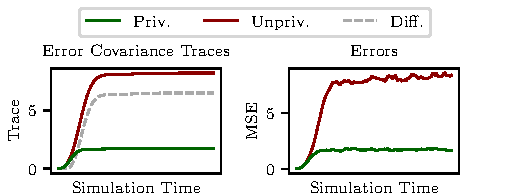
\includegraphics{figures/single_level_bounded.pdf}
   \caption{Privileged estimation with bounded error covariance.}
   \label{fig:single_bounded}
\end{figure}

The second simulation considers an unobservable system where only the velocity is measured and has an unbounded error covariance as $k \rightarrow \infty$. It is given by 
$
   \mat{H}_k=
   \begin{bsmallmatrix}
      0 & 1 & 0 & 0\\
      0 & 0 & 0 & 1
   \end{bsmallmatrix}
$, 
for all $k$, and uses the same values for $\mat{R}_k$ and $\mat{Z}$ as the previous model. Figure \ref{fig:single_unbounded} shows the average error covariance traces and MSE of estimation from 1000 runs using this model and captures how error covariance boundedness does not affect the privileged estimation scheme's properties.

\begin{figure}[htbp]
   \centering
   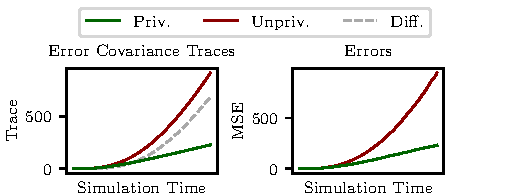
\includegraphics{figures/single_level_unbounded.pdf}
   \caption{Privileged estimation with unbounded error covariance.}
   \label{fig:single_unbounded}
\end{figure}

Lastly, a simulation of multiple privilege levels was also performed using the bounded error covariance measurement model and using pseudorandom Gaussian samples such that $\mat{E}_1=20 \cdot \mat{I}$, $\mat{E}_2=14 \cdot \mat{I}$, and $\mat{E}_3=17 \cdot \mat{I}$ for estimators holding the single keys $\mathsf{sk}_1$, $\mathsf{sk}_2$ and $\mathsf{sk}_3$, respectively. Note that the three matrices $\mat{E}_i$, $1 \leq i \leq 3$ satisfy \eqref{eqn:mult_covariance_restriction}. Figure \ref{fig:multiple_bounded} again shows the average traces and MSE of estimation from 1000 runs and displays the distinct difference in estimation error of the different privilege levels. Additionally, two special cases that bound all estimators are included, one holding all privilege level keys and another holding none.

\begin{figure}[htbp]
   \centering
   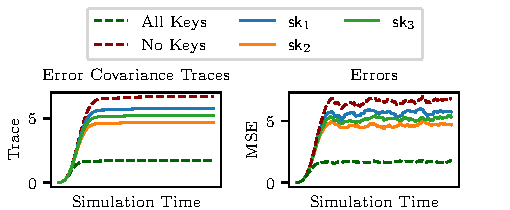
\includegraphics{figures/multiple_level.pdf}
   \caption{Estimation with multiple privilege levels.}
   \label{fig:multiple_bounded}
\end{figure}

All of the included figures capture the difference in estimation error between the best possible estimators given the simulated processes (in terms of MSE) and support the proposed security proof sketch given in section [sec:scheme\_security].


% 
% 8888888b.  8888888b.  8888888 888     888      8888888888 888     888  .d8888b.  8888888888 
% 888   Y88b 888   Y88b   888   888     888      888        888     888 d88P  Y88b 888        
% 888    888 888    888   888   888     888      888        888     888 Y88b.      888        
% 888   d88P 888   d88P   888   Y88b   d88P      8888888    888     888  "Y888b.   8888888    
% 8888888P"  8888888P"    888    Y88b d88P       888        888     888     "Y88b. 888        
% 888        888 T88b     888     Y88o88P        888        888     888       "888 888        
% 888        888  T88b    888      Y888P         888        Y88b. .d88P Y88b  d88P 888        
% 888        888   T88b 8888888     Y8P          888         "Y88888P"   "Y8888P"  8888888888 
%                                                                                             
%                                                                                             
%                                                                                             
% 

\section{Fusion in Privileged Estimation Environments}\label{sec:priv_estimation:privileged_fusion}
The idea behind our privileged fusion scheme is to add \textit{correlated} Gaussian keystreams to the measurements from each sensor. These noises can be computed and subtracted by estimators holding respective sensor keys, while their correlation limits the additional information gained from fusing unprivileged measurements. 

% 
%  ######   #######  ########  ########     ##    ## ######## ##    ##  ######  
% ##    ## ##     ## ##     ## ##     ##    ##   ##  ##        ##  ##  ##    ## 
% ##       ##     ## ##     ## ##     ##    ##  ##   ##         ####   ##       
% ##       ##     ## ########  ########     #####    ######      ##     ######  
% ##       ##     ## ##   ##   ##   ##      ##  ##   ##          ##          ## 
% ##    ## ##     ## ##    ##  ##    ##     ##   ##  ##          ##    ##    ## 
%  ######   #######  ##     ## ##     ##    ##    ## ########    ##     ######  
% 

\subsection{Correlated Gaussian Keystreams}\label{subsec:priv_estimation:fus_gaussian_keystreams}
Similarly to the Gaussian keystream generation in [eqn:gaussian\_keystream\_generation], pseudorandom samples can be correlated in this way even when generated using different stream cipher keys. To parameterise the correlation between noises at each sensor, we introduce a fully correlated component $\mat{Z}\in\mathbb{R}^{m\times m}$ and an uncorrelated component $\mat{Y}\in\mathbb{R}^{m\times m}$ and define a noise cross-correlation matrix for $x$ noises as $\mat{S}^{(x)} \in \mathbb{R}^{xm\times xm}$,
\begin{equation}\label{eqn:noise_correlation_matrix}
  \mat{S}^{(x)}=
  \begin{bmatrix}
    \mat{Z} & \cdots & \mat{Z}\\
    \vdots & \ddots & \vdots\\
    \mat{Z} & \cdots & \mat{Z}\\
  \end{bmatrix}+
  \begin{bmatrix}
    \mat{Y} & \mat{0} & \mat{0}\\
    \mat{0} & \ddots & \mat{0}\\
    \mat{0} & \mat{0} & \mat{Y}\\
  \end{bmatrix}\,,
\end{equation}
and $\mat{S}^{(1)}=\mat{Z}+\mat{Y}$. The generation of all $N$ multivariate Gaussian noises at timestep $k$, $\vec{g}_k^{(1:N)}$, can now be written as
\begin{equation}\label{eqn:all_correlated_noises_generation}
  \vec{g}_k^{(1:N)}=
  \begin{bmatrix}
    \vec{g}_{k,1}\\
    \vdots\\
    \vec{g}_{k,N}
  \end{bmatrix}=
  \mat{S}^{(N)\frac{1}{2}}\cdot
  \begin{bmatrix}
    \vec{z}_{k,1}\\
    \vdots\\
    \vec{z}_{k,N}
  \end{bmatrix}\,,
\end{equation}
where each $\vec{z}_{k,i}$ is computed as $\vec{z}_k$ in [eqn:standard\_gaussian\_generation] using uniform samples generated with key $\mathsf{sk}_i$, and $\mat{S}^{(N)\frac{1}{2}}$ is a matrix such that $\mat{S}^{(N)\frac{1}{2}}\mat{S}^{(N)\frac{1}{2}\top}=\mat{S}^{(N)}$. Notably, it is important that the vector of the first $p$ noises $\vec{g}_{k,i}$, $1\leq i \leq p$, in \eqref{eqn:all_correlated_noises_generation}, denoted $\vec{g}_k^{(1:p)}$, can be reproduced by an estimator of privilege $p$, holding only the keys $\mathsf{sk}_i$, $1\leq i \leq p$. One case where this is possible is when a lower-triangular decomposition, such as the Cholesky decomposition, is used to compute $\mat{S}^{(N)\frac{1}{2}}$ from $\mat{S}^{(N)}$. Here, each correlated Gaussian sample $\vec{g}_{k,i}$ is computable from preceeding uniform samples $\vec{z}_{k,j}$, $j\leq i$ only, and the generalised noise generation equation
\begin{equation}\label{eqn:p_correlated_noises_generation}
  \vec{g}_k^{(1:p)}=
  \mat{S}^{(p)\frac{1}{2}}\cdot
  \begin{bmatrix}
    \vec{z}_{k,1}\\
    \vdots\\
    \vec{z}_{k,p}
  \end{bmatrix}
\end{equation}
generates the same first $p$ noises $\vec{g}_k^{(1:p)}$ as would be obtained from \eqref{eqn:all_correlated_noises_generation}. This is due to $\mat{S}^{(p)\frac{1}{2}}\in\mathbb{R}^{pm\times pm}$ equalling the top left block of matrix $\mat{S}^{(N)\frac{1}{2}}$ when using a lower-triangular decomposition.

With \eqref{eqn:p_correlated_noises_generation}, at every timestep $k$, $\vec{g}_k^{(1:N)}$ can be generated using all $N$ keys and used to modify sensor measurements, while the subset $\vec{g}_k^{(1:p)}$ can be generated by estimators of privilege $p$ using only the keys they hold.

% 
% ##     ##  #######  ########  
% ###   ### ##     ## ##     ## 
% #### #### ##     ## ##     ## 
% ## ### ## ##     ## ##     ## 
% ##     ## ##     ## ##     ## 
% ##     ## ##     ## ##     ## 
% ##     ##  #######  ########  
% 

\subsection{Measurement Modification}\label{subsec:priv_estimation:fus_measurement_mod}
With a way to generate noises for sensors and estimators, we can introduce the means of measurement modification and the observable measurement models for different estimators. Measurement modification is peformed by adding noises $\vec{g}_k^{(1:N)}$ to measurements from each sensor $i$ before making them public, resulting in modified measurement equations for each sensor,
\begin{equation}\label{eqn:modified_measurement_priv2}
\begin{split}
  \vec{y}_{k,i}^\prime &= \vec{y}_{k,i} + \vec{g}_{k,i}\\
  &= \mat{H}_{k,i}\vec{x}_k + \vec{v}_{k,i} + \vec{g}_{k,i}\,,
\end{split}
\end{equation}
with real measurement noise $\vec{v}_{k,i}\sim\mathcal{N}(\vec{0},\mat{R}_{k,i})$ and the vector of all added noises $\vec{g}_k^{(1:N)}\ \dot{\sim}\ \mathcal{N}(\vec{0}, \mat{S}^{(N)})$. As we assume that sensors are synchronised in $k$, we can capture the correlation between these modified measurements exactly by considering the stacked measurement model for any estimator with access to $q$ measurements, $\mathsf{e}^{[p,q]}$, at time $k$, given by
\begin{equation}\label{eqn:measurement_equation}
  \begin{split}
    \vec{y}_k^{\prime(1:q)} &= \vec{y}_k^{(1:q)} + \vec{g}_k^{(1:q)}\\
    &= \mat{H}_k^{(1:q)}\vec{x}_k + \vec{v}_k^{(1:q)} + \vec{g}_k^{(1:q)}
  \end{split}
\end{equation}
where $\vec{v}_k^{(1:q)}\sim\mathcal{N}(\vec{0},\mat{R}_k^{(1:q)})$ and $\vec{g}_k^{(1:q)}\ \dot{\sim}\ \mathcal{N}(\vec{0},\mat{S}^{(q)})$, with
\begin{equation*}
  \vec{y}_k^{\prime(1:q)}=
  \begin{bmatrix}
    \vec{y}_{k,1}^\prime\\
    \vdots\\
    \vec{y}_{k,q}^\prime
  \end{bmatrix},\ 
  \vec{y}_k^{(1:q)}=
  \begin{bmatrix}
    \vec{y}_{k,1}\\
    \vdots\\
    \vec{y}_{k,q}
  \end{bmatrix},\ 
  \mat{H}_k^{(1:q)}=
  \begin{bmatrix}
    \mat{H}_{k,1}\\
    \vdots\\
    \mat{H}_{k,q}\\
  \end{bmatrix}\,,
\end{equation*}
\begin{equation*}
  \vec{v}_k^{(1:q)}=
  \begin{bmatrix}
    \vec{v}_{k,1}\\
    \vdots\\
    \vec{v}_{k,q}
  \end{bmatrix},\ 
  \mat{R}_k^{(1:q)}=
    \begin{bmatrix}
      \mat{R}_{k,1} & \mat{0} & \mat{0}\\
      \mat{0} & \ddots & \mat{0}\\
      \mat{0} & \mat{0} & \mat{R}_{k,q}
    \end{bmatrix}\,
\end{equation*}
and $\mat{S}^{(q)} \in \mathbb{R}^{qm\times qm}$ defined by \eqref{eqn:noise_correlation_matrix}.

Since we are using a cryptographically sound stream cipher to generate the added Gaussian keystream, the pseudorandom samples are indistinguishable from truly random ones to estimators without appropriate keys, which leads us to three observable measurement models, \textit{i.e.}, the models that capture all the information available to an estimator exactly, for three types of mutually exhaustive estimators.
\begin{description}
  \item[Estimators of the form $\mathsf{e}^{[0,q]}$] Here, no keys are held by an unprivileged estimator with access to $q$ measurements, thus all generated noises $\vec{g}_k^{(1:q)}$ are indistinguishable from noises from the truly random distribution $\mathcal{N}(\vec{0}, \mat{S}^{(q)})$. For these estimators, we can rewrite the measurement equation \eqref{eqn:measurement_equation} as the observed measurement model
  \begin{equation}\label{eqn:0q_obs_measurement_model}
    \vec{y}_k^{[0,q]} = \mat{H}_k^{(1:q)}\vec{x}_k + \vec{v}_k^{\prime}\,,
  \end{equation}
  with truly Gaussian term $\vec{v}_k^{\prime} \sim \mathcal{N}(\vec{0}, \mat{R}_k^{(1:q)}+\mat{S}^{(q)})$.
  
  \item[Estimators of the form $\mathsf{e}^{[p,p]}$] Estimators with keys for all the sensors to which they have access can generate all added noises and subtract them from the received measurements. That is, $\vec{g}_k^{(1:p)}$ can be generated and $\vec{y}_k^{[p,p]}=\vec{y}_k^{\prime(1:p)}-\vec{g}_k^{(1:p)}$ computed to give the observed measurement model equal to recieving unmodified measurements only,
  \begin{equation}\label{eqn:pp_obs_measurement_model}
    \vec{y}_k^{[p,p]} = \mat{H}_k^{(1:p)}\vec{x}_k + \vec{v}_k^{(1:p)}\,,
  \end{equation}
  where $\vec{v}_k^{(1:p)} \sim \mathcal{N}(\vec{0}, \mat{R}_k^{(1:p)})$.

  \item[Estimators of the form $\mathsf{e}^{[p,q]}$, $p<q$] Lastly, we want the observed measurement model when only some accessible measurements can have their noises removed. Here, the noises from sensors $i>p$ which cannot be removed are conditionally dependent on the known noises $\vec{g}_k^{(1:p)}$. Since we can generate the noises $\vec{g}_k^{(1:p)}$ and know that $\vec{g}_k^{(1:q)}\ \dot{\sim}\ \mathcal{N}(\vec{0}, \mat{S}^{(q)})$, we can write 
  \begin{equation}\label{eqn:block_noises_and_correlation}
    \begin{split}
      &\vec{g}_k^{(1:q)}=
      \begin{bmatrix}
        \vec{g}_k^{(1:p)}\\
        \vec{g}_k^{(p+1:q)}\\
      \end{bmatrix}\\ 
      &\qquad \dot{\sim}\ \mathcal{N}\left(
      \begin{bmatrix}
        \vec{0}\\
        \vec{0}
      \end{bmatrix},
      \begin{bmatrix}
        \mat{S}^{(p)} & \bar{\mat{Z}}\\
        \bar{\mat{Z}}^\top & \mat{S}^{(q-p)}
      \end{bmatrix}\right)\,,
    \end{split}
  \end{equation}
  where $\bar{\mat{Z}} \in \mathbb{R}^{pm \times (q-p)m}$ is a block matrix with every block equal to $\mat{Z}$, and compute the conditional pseudorandom Gaussian distribution
  \begin{equation}\label{eqn:conditional_noise_distribution}
    \begin{split}
      &\vec{g}_k^{(p+1:q)} \mid \vec{g}_k^{(1:p)}\\
      &\qquad \dot{\sim}\ \mathcal{N}\Big(\bar{\mat{Z}}^\top\mat{S}^{(p)-1}\vec{g}_k^{(1:p)},\\
      &\qquad\qquad \mat{S}^{(q-p)} - \bar{\mat{Z}}^\top\mat{S}^{(p)-1}\bar{\mat{Z}}\Big)\,.
    \end{split}
  \end{equation}
  Now, subtracting the known noises $\vec{g}_k^{(1:p)}$ and the means of the unknown noises \eqref{eqn:conditional_noise_distribution} from recieved measurements,
  \begin{equation}\label{eqn:pq_measurement_offset}
    \vec{y}_k^{[p,q]}=\vec{y}_k^{\prime(1:q)} - 
    \begin{bmatrix}
      \vec{g}_k^{(1:p)}\\
      \bar{\mat{Z}}^\top\mat{S}^{(p)-1}\vec{g}_k^{(1:p)}
    \end{bmatrix}\,,
  \end{equation}
  and accounting for unknown pseudorandom noises being indistinguishable from random, a zero-mean observed measurement model can be written as
  \begin{equation}\label{eqn:pq_obs_measurement_model}
    \vec{y}_k^{[p,q]} = \mat{H}_k^{(1:q)}\vec{x}_k + \vec{v}_k^{\prime}
  \end{equation}
  where 
  \begin{equation*}
    \begin{split}
      &\vec{v}_k^{\prime} \sim \mathcal{N}\Bigg(\vec{0},\\
      &\qquad 
      \begin{bmatrix}
        \mat{R}_k^{(1:p)} & \mat{0}\\
        \mat{0} & \mat{S}^{(q-p)} - \bar{\mat{Z}}^\top\mat{S}^{(p)-1}\bar{\mat{Z}} + \mat{R}_k^{(p+1:q)}
      \end{bmatrix}\Bigg).
    \end{split}
  \end{equation*}
\end{description}
\begin{remark}
  Recalling that we assume estimators access unprivileged measurements sequentially to simplify notation, \eqref{eqn:block_noises_and_correlation}, \eqref{eqn:pq_measurement_offset} and \eqref{eqn:pq_obs_measurement_model} can be generalised when having access to arbitrary $q-p$ non-sequential unprivileged measurements $\vec{y}_{k,i}$, $p<i\leq q$, by appropriately rearranging the columns of $\mat{S}^{(q-p)}$ in \eqref{eqn:block_noises_and_correlation}.
\end{remark}

From the observed measurement models \eqref{eqn:0q_obs_measurement_model}, \eqref{eqn:pp_obs_measurement_model} and \eqref{eqn:pq_obs_measurement_model} we can tell that the parameters $\mat{Z}$ and $\mat{Y}$ (within matrices $\mat{S}^{(q)}$, $\mat{S}^{(p)}$ and $\mat{S}^{(q-p)}$) will control the difference in estimation performance between the three types of estimators. Computing the two differences we wish to cryptographically guarantee from section [sec:prob], and how $\mat{Z}$ and $\mat{Y}$ affect them, will be more formally explored in sections [sec:crypto] and [sec:sim].

% 
% ##    ##  #######  ####  ######  ########    ########  ####  ######  ######## 
% ###   ## ##     ##  ##  ##    ## ##          ##     ##  ##  ##    ##    ##    
% ####  ## ##     ##  ##  ##       ##          ##     ##  ##  ##          ##    
% ## ## ## ##     ##  ##   ######  ######      ##     ##  ##   ######     ##    
% ##  #### ##     ##  ##        ## ##          ##     ##  ##        ##    ##    
% ##   ### ##     ##  ##  ##    ## ##          ##     ##  ##  ##    ##    ##    
% ##    ##  #######  ####  ######  ########    ########  ####  ######     ##    
% 

\subsection{Distribution of Noise Terms}\label{subsec:priv_estimation:fus_noise_dist}
While we have described a method for generating noises that modify $N$ measurements and result in different observed measurement models depending on estimator privilege, we have not discussed where the noise is generated and how it is distributed to sensors. To handle the inherent correlation of the noises $\vec{g}_{k}^{(1:N)}$, they can be generated either centrally before distribution to sensors or sequentially at the sensors themselves, given previously generated values.
\begin{description}
  \item[Central noise generation] To compute noises centrally, \eqref{eqn:p_correlated_noises_generation} can be computed for all $N$ noises at a central processor and each noise $\vec{g}_{k,i}$ sent to the respective sensor $i$ before it modifies its local measurement by \eqref{eqn:modified_measurement_priv2}.
  \item[Sequential noise generation] To compute the same noises sequentially for each timestep $k$, sensor $1$ can generate its noise independently using its current standard Gaussian sample $\vec{z}_{k,1}$, by $\vec{g}_{k,1} = \mat{S}^{(1)\frac{1}{2}}\vec{z}_{k,1}$. Each following sensor $i>1$ can generate its noise $\vec{g}_{k,i}$ given the preceeding noises $\vec{g}_k^{(1:i-1)}$ and following the conditional reasoning in \eqref{eqn:conditional_noise_distribution}, as
  \begin{equation}
    \begin{split}
      \vec{g}_{k,i} = &\bar{\mat{Z}}^\top\mat{S}^{(i-1)-1}\vec{g}_k^{(1:i-1)} +\\
      &\qquad (\mat{S}^{(1)}-\bar{\mat{Z}}^\top\mat{S}^{(i-1)-1}\bar{\mat{Z}})^\frac{1}{2}\vec{z}_{k,i}\,.
    \end{split}
  \end{equation}
  After local noise generation, sensor $i$ sends its and preceding noises, $\vec{g}_k^{(1:i)}$, to the next sensor $i+1$. This method has the clear downside of increasing communication costs with each successive generation but requires no central communicator.
\end{description}
In both cases above, the computation of all noises $\vec{g}_k^{(1:N)}$ can be performed offline, reducing the complexity of real-time measurement modification.

% 
%  ######  ########  ##    ## ########  ########  #######  
% ##    ## ##     ##  ##  ##  ##     ##    ##    ##     ## 
% ##       ##     ##   ####   ##     ##    ##    ##     ## 
% ##       ########     ##    ########     ##    ##     ## 
% ##       ##   ##      ##    ##           ##    ##     ## 
% ##    ## ##    ##     ##    ##           ##    ##     ## 
%  ######  ##     ##    ##    ##           ##     #######  
% 
\subsection{Security Analysis}\label{subsec:priv_estimation:fus_security}
To give proof sketches of the cryptographic guarantees provided by the presented scheme, we first recall some assumptions. We consider floating-point numbers to be sufficiently close to real random numbers that real-number proofs still hold, and that all sensors are synchronised in $k$ such that observed measurement models \eqref{eqn:0q_obs_measurement_model}, \eqref{eqn:pp_obs_measurement_model} and \eqref{eqn:pq_obs_measurement_model} are exactly correct. Using these assumptions, the proofs rely on the optimality of the linear Kalman filter (KF) [haugBayesianEstimationTracking2012] to produce a series of covariances for optimal estimators before taking their differences to obtain the \textit{Performance Loss Lower Bound} and \textit{Performance Gain Upper Bound} from section [sec:prob]. Similarly to [risticCryptographicallyPrivilegedState2022], these series can be used as $\mat{D}_1,\mat{D}_2,\dots$ in definition [def:cov\_priv\_security\_notion] for appropriately formulated privileged estimation schemes for the two bounds, and demonstrate that the existence of an estimator violating the notion implies the existence of a linear estimator with error covariance lower than the KF. This guarantees the bounds by contrapositive.

% 
% .##........#######...######...######.....########...#######..##.....##.##....##.########.
% .##.......##.....##.##....##.##....##....##.....##.##.....##.##.....##.###...##.##.....##
% .##.......##.....##.##.......##..........##.....##.##.....##.##.....##.####..##.##.....##
% .##.......##.....##..######...######.....########..##.....##.##.....##.##.##.##.##.....##
% .##.......##.....##.......##.......##....##.....##.##.....##.##.....##.##..####.##.....##
% .##.......##.....##.##....##.##....##....##.....##.##.....##.##.....##.##...###.##.....##
% .########..#######...######...######.....########...#######...#######..##....##.########.
% 

\subsubsection{Performance Loss Lower Bound (PLLB)}
First, we consider the lower bound to the loss in estimation performance an estimator $\mathsf{e}^{[0,N]}$ has on an estimator $\mathsf{e}^{[p,p]}$ when measurements follow the presented scheme. Since the observed measurement models for these estimators, \eqref{eqn:0q_obs_measurement_model} and \eqref{eqn:pp_obs_measurement_model}, interpret available measurements as a single stacked measurement, and since we do not consider estimators that corrupt sensors, we can treat the stacked measurement as coming from a single sensor and use the notion of covariance privilege in definition [def:cov\_priv\_security\_notion] to guarantee the bound. The associated privileged estimation scheme for the PLLB can be written for each privilege $p$ as
\begin{description}
  \item[$\mathsf{Setup}$] Given the system model \eqref{eqn:system_model_priv}, all measurements models \eqref{eqn:measurement_models} (interpretable as a single stacked measurement model) and a security parameter $\kappa$ used by all sensors, generate $N$ stream cipher keys $\mathsf{sk_i}$, $1\leq i \leq N$, and let the secret key $\mathsf{sk}$ include all $N$ keys. Generate the correlated and uncorrelated noise components $\mat{Z}$ and $\mat{Y}$, an initial estimate and error covariance $\hat{\vec{x}}_0$ and $\mat{P}_0$, and include these in the public parameters $\mathsf{pub}$.
  
  \item[$\mathsf{Noise}_{\mathsf{PLLB}}$] Given parameters, cipher keys, a timestep $k$ and true sensor measurements $\vec{y}_k^{(1:N)}$, let $\vec{y}_k^{\{\mathsf{up}\}}=\vec{y}_k^{[0,N]}$ following \eqref{eqn:0q_obs_measurement_model} and $\vec{y}_k^{\{\mathsf{p}\}}=\vec{y}_k^{[p,p]}$ following \eqref{eqn:pp_obs_measurement_model}.
\end{description}
With the above formulation, we can use the KF to recursively compute the optimal estimate error covariances for estimators with access to only measurements $\vec{y}_k^{\{\mathsf{up}\}}$ or $\vec{y}_k^{\{\mathsf{p}\}}$, for all $k$. Since the KF preserves initial covariance order, $\mat{P}_k \succeq \mat{P}_k^\prime \implies \mat{P}_{k+1} \succeq \mat{P}_{k+1}^\prime$, a lower bound can be guaranteed when using the initial covariance $\mat{P}_0=\mat{0}$. Therefore, the minimum achievable error covariance for an estimator $\mathsf{e}^{[0,N]}$, with access to measurements $\vec{y}_k^{\{\mathsf{up}\}}=\vec{y}_k^{[0,N]}$, is given by the combined KF predict and update equations
\begin{equation}\label{eqn:0N_lower_bound_covariance}
  \begin{split}
    \mat{P}_k^{[0,N]} =& \Bigl( \mat{I} - (\mat{F}_k\mat{P}_{k-1}^{[0,N]}\mat{F}_k^\top + \mat{Q}_k)\mat{H}_k^{(1:N)\top} \cdot \\
    &\quad\bigl(\mat{H}_k^{(1:N)}(\mat{F}_k\mat{P}_{k-1}^{[0,N]}\mat{F}_k^\top + \mat{Q}_k)\mat{H}_k^{(1:N)\top} \\
    &\quad+ \mat{R}_k^{(1:N)} + \mat{S}^{(N)}\bigr)^{-1}\mat{H}_k^{(1:N)}\Bigr)\cdot\\
    &\Bigl(\mat{F}_k\mat{P}_{k-1}^{[0,N]}\mat{F}_k^\top + \mat{Q}_k\Bigr)\,,
 \end{split}
\end{equation}
when $\mat{P}_0^{[0,N]}=\mat{0}$. Similarly, the same can be done for an estimator $\mathsf{e}^{[p,p]}$, with access to measurements $\vec{y}_k^{\{\mathsf{p}\}}=\vec{y}_k^{[p,p]}$, as
\begin{equation}\label{eqn:pp_lower_bound_covariance}
  \begin{split}
    \mat{P}_k^{[p,p]} =& \Bigl( \mat{I} - (\mat{F}_k\mat{P}_{k-1}^{[p,p]}\mat{F}_k^\top + \mat{Q}_k)\mat{H}_k^{(1:p)\top} \cdot \\
    &\quad\bigl(\mat{H}_k^{(1:p)}(\mat{F}_k\mat{P}_{k-1}^{[p,p]}\mat{F}_k^\top + \mat{Q}_k)\mat{H}_k^{(1:p)\top} \\
    &\quad+ \mat{R}_k^{(1:p)}\bigr)^{-1}\mat{H}_k^{(1:p)}\Bigr)\cdot\\
    &\Bigl(\mat{F}_k\mat{P}_{k-1}^{[p,p]}\mat{F}_k^\top + \mat{Q}_k\Bigr)
  \end{split}
\end{equation}
and $\mat{P}_0^{[p,p]}=\mat{0}$. The bounds \eqref{eqn:0N_lower_bound_covariance} and \eqref{eqn:pp_lower_bound_covariance} are constructed such that at every timestep $k$,
\begin{equation}\label{eqn:0N_cov_bound}
  \begin{split}
    &\mat{P}_k^{[0,N]} \preceq\\
    &\qquad \mathsf{Cov}\left[\mathcal{A}\left(k,\mathcal{M}_S,\mathcal{M}_M,\vec{y}_1^{[0,N]},\dots,\vec{y}_k^{[0,N]}\right) - \vec{x}_k\right]
  \end{split}
\end{equation}
and
\begin{equation}\label{eqn:pp_cov_bound}
  \begin{split}
    &\mat{P}_k^{[p,p]} \preceq\\
    &\qquad \mathsf{Cov}\left[\mathcal{A}\left(k,\mathcal{M}_S,\mathcal{M}_M,\vec{y}_1^{[p,p]},\dots,\vec{y}_k^{[p,p]}\right) - \vec{x}_k\right]
  \end{split}
\end{equation}
hold. Recalling definition [def:cov\_priv\_security\_notion], and knowing that the minimum achievable covariance of the estimators is produced using the KF, it can be seen that the difference 
\begin{equation}\label{eqn:unpriv_priv_pllb_difference_series}
  \mat{D}_{\mathsf{PLLB},k} = \mat{P}_k^{[0,N]} - \mat{P}_k^{[p,p]}\,
\end{equation}
produces a series where for any PPT estimator $\mathsf{e}^{[0,N]}$, an equivalent PPT estimator $\mathsf{e}^{[p,p]}$, lower bounded in error by \eqref{eqn:pp_lower_bound_covariance}, can always be created such that the difference between their error covariances at time $k$ is at least $\mat{D}_{\mathsf{PLLB},k}$. Here, the PPT requirement guarantees the indistinguishabilty of pseudorandom streams to truly random ones and a negligible performance gain for $\mathsf{e}^{[0,N]}$ is present on average if secret keys or keystreams are guessed. The existence of an estimator of the form $\mathsf{e}^{[0,N]}$ where this condition cannot be met, implies the existence of an estimator with error covariances smaller than the KF for linear models. As no such estimator exists, we conclude that the $\mathsf{Setup}$ and $\mathsf{Noise_{\mathsf{PLLB}}}$ algorithms above meet \textit{$\{\mat{D}_{\mathsf{PLLB},1},\mat{D}_{\mathsf{PLLB},2},\dots\}$-Covariance Privilege for System Model \eqref{eqn:system_model_priv} and Stacked Measurement Models \eqref{eqn:measurement_models}}.

In the above, we lower bound the estimation performance loss an estimator $\mathsf{e}^{[0,N]}$ has on estimators $\mathsf{e}^{[p,p]}$. In the cases where the unprivileged estimator has access to fewer measurements, $\mathsf{e}^{[0,q]}$, $q<N$, or the privileged one to more, $\mathsf{e}^{[p,q]}$, $q>p$, the achievable difference can only increase (fewer measurements can only increase error covariance while more can only decrease it). This ensures the computed bound remains a lower bound for \textit{any} unprivileged estimator.

% 
% ..######......###....####.##....##....########...#######..##.....##.##....##.########.
% .##....##....##.##....##..###...##....##.....##.##.....##.##.....##.###...##.##.....##
% .##.........##...##...##..####..##....##.....##.##.....##.##.....##.####..##.##.....##
% .##...####.##.....##..##..##.##.##....########..##.....##.##.....##.##.##.##.##.....##
% .##....##..#########..##..##..####....##.....##.##.....##.##.....##.##..####.##.....##
% .##....##..##.....##..##..##...###....##.....##.##.....##.##.....##.##...###.##.....##
% ..######...##.....##.####.##....##....########...#######...#######..##....##.########.
% 

\subsubsection{Performance Gain Upper Bound (PGUB)}
Similar to the lower bound above, we can use the same properties of the KF to give an upper bound to the gain in estimation performance an estimator $\mathsf{e}^{[p,N]}$ has on an estimator $\mathsf{e}^{[p,p]}$ when measurements follow the presented scheme. The associated privileged estimation scheme for the PGUB for each privilege $p$ is given by the same $\mathsf{Setup}$ algorithm as in section [subsec:crypto\_performance\_loss\_lower\_bound] and
\begin{description}
  \item[$\mathsf{Noise}_{\mathsf{PGUB}}$] Given parameters, cipher keys, a timestep $k$ and true sensor measurements $\vec{y}_k^{(1:N)}$, let $\vec{y}_k^{\{\mathsf{up}\}}=\vec{y}_k^{[p,N]}$ following \eqref{eqn:pq_obs_measurement_model} and $\vec{y}_k^{\{\mathsf{p}\}}=\vec{y}_k^{[p,p]}$ following \eqref{eqn:pp_obs_measurement_model}.
\end{description}
The minimum error covariances achievable by an estimator $\mathsf{e}^{[p,p]}$ is again given by \eqref{eqn:pp_lower_bound_covariance} and $\mat{P}_0^{[p,p]} = \mat{0}$. For an estimator $\mathsf{e}^{[p,N]}$ with access to measurements $\vec{y}_k^{\{\mathsf{up}\}}=\vec{y}_k^{[p,N]}$ it is given by
\begin{equation}\label{eqn:pN_lower_bound_covariance}
  \begin{split}
    \mat{P}_k^{[p,N]} =& \Bigl( \mat{I} - (\mat{F}_k\mat{P}_{k-1}^{[p,N]}\mat{F}_k^\top + \mat{Q}_k)\mat{H}_k^{(1:N)\top} \cdot \\
    &\quad\bigl(\mat{H}_k^{(1:N)}(\mat{F}_k\mat{P}_{k-1}^{[p,N]}\mat{F}_k^\top + \mat{Q}_k)\mat{H}_k^{(1:N)\top} \\
    &\quad+ \mat{X}\bigr)^{-1}\mat{H}_k^{(1:N)}\Bigr)\Bigl(\mat{F}_k\mat{P}_{k-1}^{[p,N]}\mat{F}_k^\top + \mat{Q}_k\Bigr)\,,
 \end{split}
\end{equation}
where
\begin{equation}
  \mat{X} = 
  \begin{bmatrix}
    \mat{R}_k^{(1:p)} & \mat{0}\\
    \mat{0} & \mat{S}^{(N-p)} - \bar{\mat{Z}}^\top\mat{S}^{(p)-1}\bar{\mat{Z}} + \mat{R}_k^{(p+1:N)}
  \end{bmatrix}
\end{equation}
and $\mat{P}_0^{[p,N]} = \mat{0}$. Again, the bounding series are such that \eqref{eqn:pp_cov_bound} and
\begin{equation}\label{eqn:pN_cov_bound}
  \begin{split}
    &\mat{P}_k^{[p,N]} \preceq\\
    &\qquad \mathsf{Cov}\left[\mathcal{A}\left(k,\mathcal{M}_S,\mathcal{M}_M,\vec{y}_1^{[p,N]},\dots,\vec{y}_k^{[p,N]}\right) - \vec{x}_k\right]
  \end{split}
\end{equation}
hold. Now, the difference
\begin{equation}\label{eqn:unpriv_priv_pgub_difference_series}
  \mat{D}_{\mathsf{PGUB},k} = \mat{P}_k^{[p,N]} - \mat{P}_k^{[p,p]}\,
\end{equation}
produces a series where for any PPT estimator $\mathsf{e}^{[p,N]}$, an equivalent PPT estimator $\mathsf{e}^{[p,p]}$, lower bounded in error by \eqref{eqn:pp_lower_bound_covariance}, can always be created such that the difference between their error covariances at time $k$ is at least $\mat{D}_{\mathsf{PGUB},k}$. With the same reasoning as for the lower bound, we conclude that the $\mathsf{Setup}$ and $\mathsf{Noise}_{\mathsf{PGUB}}$ algorithms above meet \textit{$\{\mat{D}_{\mathsf{PGUB},1},\mat{D}_{\mathsf{PGUB},2},\dots\}$-Covariance Privilege for System Model \eqref{eqn:system_model_priv} and Stacked Measurement Models \eqref{eqn:measurement_models}}.

In \eqref{eqn:unpriv_priv_pgub_difference_series}, $\mat{D}_{\mathsf{PGUB},k} \preceq 0$ for all $k>0$ and lower bounds the (negative) loss in performance an estimator $\mathsf{e}^{[p,N]}$ has on estimators $\mathsf{e}^{[p,p]}$. We refer to the bound as an upper bound as its negation $-\mat{D}_{\mathsf{PGUB},k}$, $k>0$, upper bounds the estimation performance gain achievable by $\mathsf{e}^{[p,N]}$ on the estimators $\mathsf{e}^{[p,p]}$, as desired in section [sec:prob]. In the case where fewer unprivileged measurements are accessible, $\mathsf{e}^{[p,q]}$, $q<N$, this gain can only decrease, keeping the upper bound valid for any estimators $\mathsf{e}^{[p,q]}$, $q>p$.

% 
% .##....##..#######..##....##.........##.......####.##....##
% .###...##.##.....##.###...##.........##........##..###...##
% .####..##.##.....##.####..##.........##........##..####..##
% .##.##.##.##.....##.##.##.##.#######.##........##..##.##.##
% .##..####.##.....##.##..####.........##........##..##..####
% .##...###.##.....##.##...###.........##........##..##...###
% .##....##..#######..##....##.........########.####.##....##
% 

\subsubsection{Non-Linear Systems}

% 
%  ######  #### ##     ## 
% ##    ##  ##  ###   ### 
% ##        ##  #### #### 
%  ######   ##  ## ### ## 
%       ##  ##  ##     ## 
% ##    ##  ##  ##     ## 
%  ######  #### ##     ## 
% 
\subsection{Simulation}\label{subsec:priv_estimation:fus_simulation}
In addition to showing how the estimation performance loss and gain bounds can be computed, we have simulated optimal estimators to demonstrate the effects of the correlated and uncorrelated components, $\mat{Z}$ and $\mat{Y}$, respectively. The state of an aircraft $\begin{bmatrix}x & y & v_x & v_y\end{bmatrix}^\top$, capturing its position $x$, $y$ (m) and velocity $v_x$, $v_y$ (m/s), was simulated following a constant velocity system model given by \eqref{eqn:system_model_priv} with parameters
\begin{equation}
  \mat{F}_k=
  \begin{bmatrix}
     1 & 0.5 & 0 & 0\\
     0 & 1 & 0 & 0\\
     0 & 0 & 1 & 0.5\\
     0 & 0 & 0 & 1
  \end{bmatrix}\,,
\end{equation}
and
\begin{equation}
  \mat{Q}_k=10^{-3}\cdot
  \begin{bmatrix}
     0.42 & 1.25 & 0 & 0\\
     1.25 & 5 & 0 & 0\\
     0 & 0 & 0.42 & 1.25\\
     0 & 0 & 1.25 & 5
  \end{bmatrix}\,,
\end{equation}
for all $k$, and measured independently by location sensors $i$, $1\leq i \leq N=4$, following \eqref{eqn:measurement_models} with constant parameters
\begin{equation}
  \mat{H}_{k,i}=
  \begin{bmatrix}
     1 & 0 & 0 & 0\\
     0 & 0 & 1 & 0
  \end{bmatrix}
  \text{ and }
  \mat{R}_{k,i}=
  \begin{bmatrix}
     5 & 2\\
     2 & 5
  \end{bmatrix}\,,
\end{equation}
for all $k$. Simulations were implemented in the Python programming language and the considered correlated and uncorrelated parameters were restricted to the forms $\mat{Z}=\Sigma_z\cdot\mat{I}$ and $\mat{Y}=\Sigma_y\cdot\mat{I}$ for simplicity. All estimators executed linear Kalman filters with the parameters above and the exact knowledge of the initial state ($\mat{P}_0=\mat{0}$).

Figure \ref{fig:mse_privs} shows the errors of different privileged estimators with access to varying sensor measurements when added noise parameters $\Sigma_z$ and $\Sigma_y$ are held constant. As would be expected, the error decreases when more keys are available, while a further decrease is achieved as more additional unprivileged measurements are fused. Here, the difference in mean squared error (MSE) between $\mathsf{e}^{[0,4]}$ and $\mathsf{e}^{[p,p]}$ (shaded blue region), and between $\mathsf{e}^{[p,p]}$ and $\mathsf{e}^{[p,4]}$ (shaded red region), are bounded on average by the trace of the PLLB series \eqref{eqn:unpriv_priv_pllb_difference_series} and PGUB series \eqref{eqn:unpriv_priv_pgub_difference_series}, respectively, when $\Sigma_z=2$ and $\Sigma_y=10$.
\begin{figure}[htbp]
  \centering
  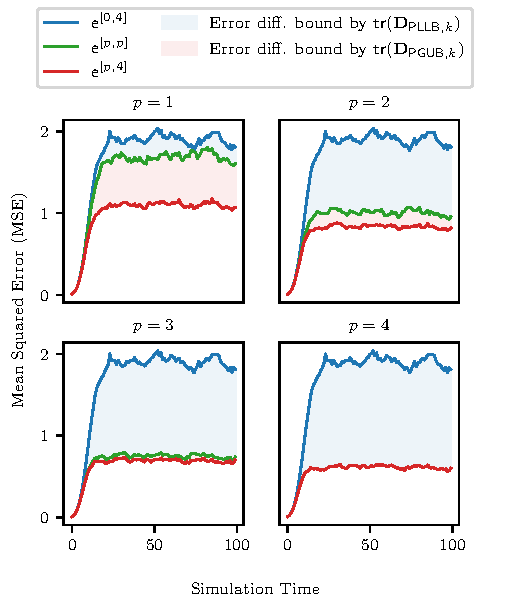
\includegraphics{figures/mse_privs.pdf}
  \caption{The average errors of different estimators for $1000$ simulation runs when $\Sigma_z=2$ and $\Sigma_y=10$.}
  \label{fig:mse_privs}
\end{figure}

To demonstrate the effect of parameters $\Sigma_z$ and $\Sigma_y$ (and therefore $\mat{Z}$ and $\mat{Y}$), figure \ref{fig:mse_params} shows their effect on the MSE given fixed estimators. It can be seen that $\Sigma_z$ has a more prominent effect on the PLLB while $\Sigma_y$ has it on the PGUB. However, it can also be observed that both parameters affect both bounds to some degree, revealing some limitations when specific bounds are desired using the proposed scheme.
\begin{figure}[htbp]
  \centering
  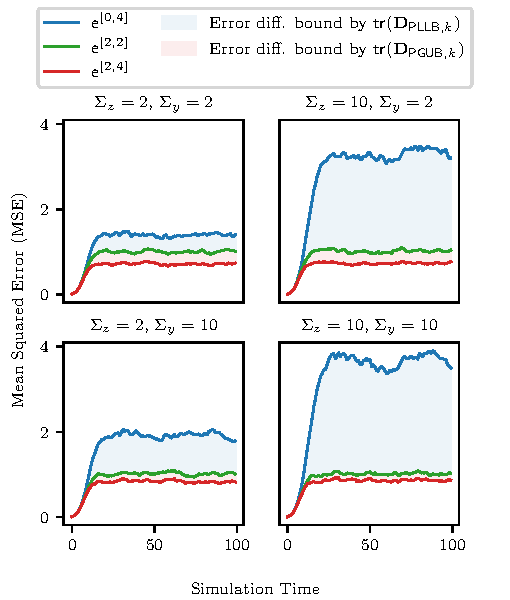
\includegraphics{figures/mse_params.pdf}
  \caption{The average errors of unprivileged and privilege-$2$ estimators for $1000$ simulation runs when varying $\Sigma_z$ and $\Sigma_y$.}
  \label{fig:mse_params}
\end{figure}
Figure \ref{fig:trace_params} further captures this relation between the bounds and the parameters $\Sigma_z$ and $\Sigma_y$. As the simulated system is asymptotically stable, steady-state error covariances are reached as $k \to \infty$, and therefore $\mat{D}_{\mathsf{PLLB},k}$ and $\mat{D}_{\mathsf{PGUB},k}$ stabilise as well. From the plot, we can see that increasing the fully correlated noise parameter $\Sigma_z$ cannot greatly reduce the PGUB (\textit{i.e.}, bring $\mathsf{tr}(\mat{D}_{\mathsf{PGUB},k})$ closer to $0$), likely due to the accurate estimation of this component by privileged estimators and the remaining uncorrelated component staying unchanged. Simultaneously, however, the fully correlated component can greatly increase the PLLB (\textit{i.e.}, take $\mathsf{tr}(\mat{D}_{\mathsf{PLLB},k})$ further from $0$) as it increases the redundancy of fusing only unprivileged measurements. The effects of increasing $\Sigma_y$ are less one-sided. The PGUB is reduced due to sufficient uncorrelated noise making the fusion of unprivileged measurements hold little information even when some keys are known, but the PLLB is increased, as uncorrelated noise still affects estimators fusing only unprivileged measurements, albeit less drastically.

Figure \ref{fig:trace_params} also shows how the bounds are affected by the privilege $p$ they are computed for. Predictably, a higher privilege results in fewer additional unprivileged measurements to fuse, lowering the PGUB, but also producing better privileged estimates, increasing the PLLB. We can also see that when the fully correlated noise term $\Sigma_z$ is small and privilege is low ($p=1$), unprivileged estimators with access to all measurements can perform better than privileged ones accessing only privileged measurements (resulting in a negative $\mathsf{tr}(\mat{D}_{\mathsf{PLLB},k})$).
\begin{figure}[htbp]
  \centering
  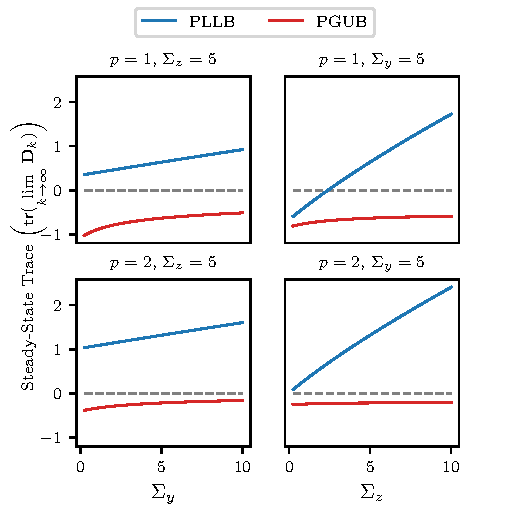
\includegraphics{figures/trace_params.pdf}
  \caption{Steady-state traces of the PLLB and PGUB for privileges $p=1$ and $p=2$ when $\Sigma_z$ and $\Sigma_y$ are varied.}
  \label{fig:trace_params}
\end{figure}

% 
%  .d8888b.   .d88888b.  888b    888  .d8888b.  
% d88P  Y88b d88P" "Y88b 8888b   888 d88P  Y88b 
% 888    888 888     888 88888b  888 888    888 
% 888        888     888 888Y88b 888 888        
% 888        888     888 888 Y88b888 888        
% 888    888 888     888 888  Y88888 888    888 
% Y88b  d88P Y88b. .d88P 888   Y8888 Y88b  d88P 
%  "Y8888P"   "Y88888P"  888    Y888  "Y8888P"  
%                                               
%                                               
%                                               
% 

\section{Conclusions on Provable Estimation Performances}\label{sec:priv_estimation:conclusion}
% In this work, we have presented the idea of a privileged estimation scheme and given a formal cryptographic definition for its security. A concrete scheme was provided that meets this notion and an intuitive extension to multiple privilege levels was discussed. A simulation demonstrating a simple use case has been presented, while the benefits of controlling estimation accuracy on a per-party basis have wide application from privatized localization hardware to subscription-based data access. Future work on the topic includes achieving formal security for broader model requirements and testing our scheme on dedicated hardware to demonstrate the method's real-time capability. 



%The presented method demonstrates how different levels of estimation performance can be cryptographically guaranteed in a network of multiple sensors. The problem considered requires sequential access to sensors and sensor keys and allows for two free parameters, $\mat{Z}$ and $\mat{Y}$, to loosely control the two relevant cryptographic bounds. The different bounds for each privilege, changing bounds over time and the relation between these parameters and the bounds themselves mean that choosing these parameters is a task-specific problem where care must be taken to meet any desired bounds without overly affecting others. The resulting cryptographic bounds can, however, always be computed exactly.

%Future work on this topic includes deriving parameters that affect the relevant cryptographic bounds independently, relaxing sequential sensor and key access requirements and exploring methods for decentralised correlated noise generation with fewer communication costs.